\documentclass[11pt, a4paper]{article}
\usepackage{graphicx}
\usepackage{amsmath}
\usepackage{listings}

\title{Assignment No 5}

\author{G Ch V Sairam , EE19B081}

\date{25-03-2021}
\begin{document}		
		
\maketitle
\section*{Introduction}

We wish to solve for the currents in a resistor. The currents depend on the shape of the resistor.

A cylindrical wire is soldered to the middle of a copper plate and its voltage
is held at 1 Volt. One side of the plate is grounded, while the remaining are
floating. The plate is 1 cm by 1 cm in size.

Combining the continuity equation and Ohm's law , we get
\begin{equation*}
 \nabla^2 \phi= 0
\end{equation*}

\section*{Assignment 5}
\subsection*{Defining parameters}
The user can give the parameters in the commandline if they want to. If no parameters are given , we use the default parameters , giving us a 25 by 25 grid with a circle of radius 8 centrally located maintained at a constant potential of 1V.We choose 1500 as the default number of iterations.
\lstinputlisting[language=Python, firstline=9, lastline=19] {EE19B081_assign5.py}

\subsection*{Initializing potential}
We start by creating an  2-D array of size Nx by Ny , consisting of all zeros. Then a list of coordinates lying within the radius is generated and these points are initialized to 1.
\lstinputlisting[language=Python, firstline=21, lastline=25]{EE19B081_assign5.py}

\begin{figure}[!tbh]
\centering
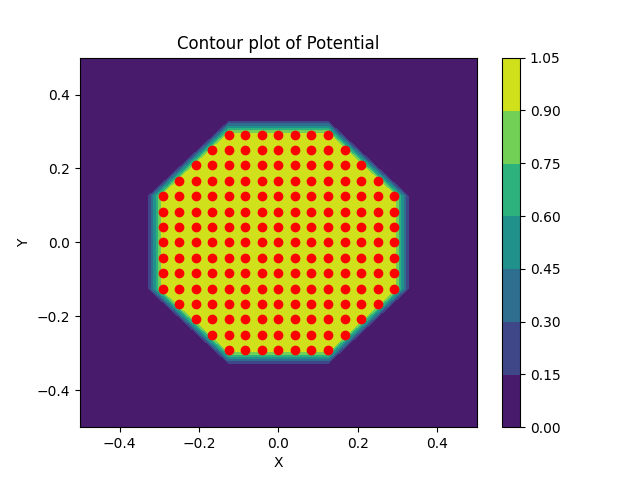
\includegraphics[scale=0.45]{Assgn5_plot1.png} 
\caption{Figure1}
\label{fig1}
\end{figure}

\subsection*{Updating potential and finding errors}
We use the difference equation to find the value of potential.
\begin{equation*}
 \phi(i,j)=0.25*[\phi(i-1,j) + \phi(i+1,j) + \phi(i,j+1) + \phi(i,j-1)]
\end{equation*}
We also assert the boundaries of the potential.

We will plot the errors on semi-log and log-log plots. We note that the error
falls really slowly and this is one of the reasons why this method of solving the Laplace equation is discouraged
\lstinputlisting[language=Python, firstline=38, lastline=48]{EE19B081_assign5.py}

\subsection*{Fitting the error and Plotting }
We note that the error is decaying exponentially for higher iterations.I have
plotted 2 fits. One considering all the iterations(fit1) and another without considering the first 500 iterations. There is very little difference between the two fits.
\lstinputlisting[language=Python, firstline=56, lastline=71]{EE19B081_assign5.py}

\begin{figure}[!tbh]
\centering
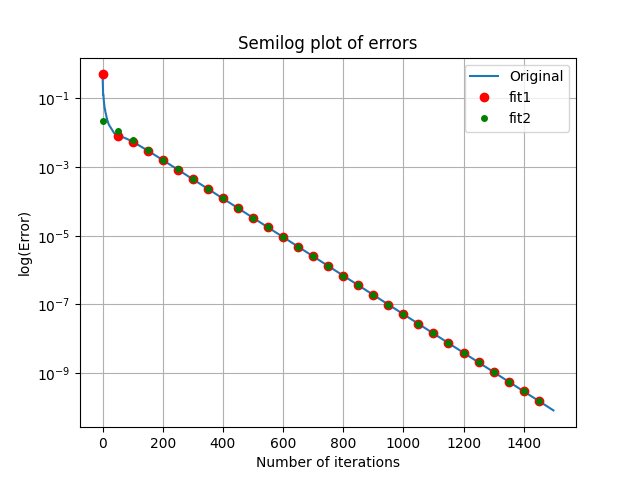
\includegraphics[scale=0.45]{Assgn5_plot2.png} 
\caption{Figure2}
\label{fig2}
\end{figure}

\begin{figure}[!tbh]
\centering
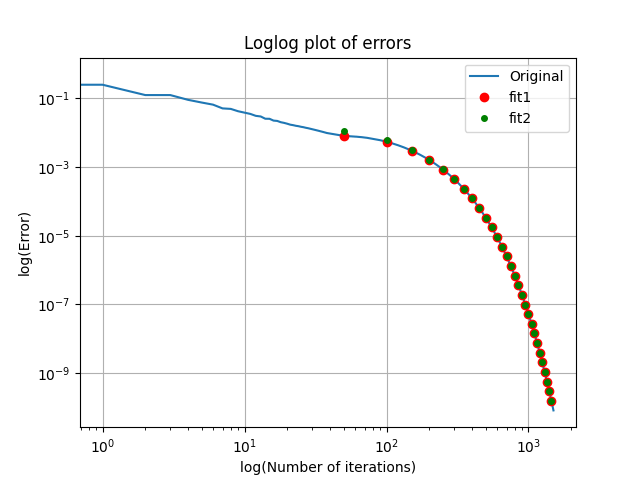
\includegraphics[scale=0.45]{Assgn5_plot3.png} 
\caption{Figure3}
\label{fig3}
\end{figure}

\begin{figure}[!tbh]
\centering
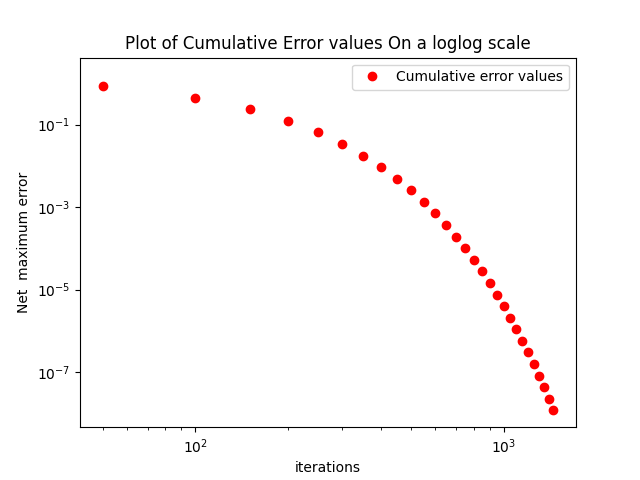
\includegraphics[scale=0.45]{Assgn5_plot4.png} 
\caption{Figure4}
\label{fig4}
\end{figure}

\subsection*{Plotting updated potentials}

There are 2 ways to plot a 3d figure.We can use the contour plot or we can plot directly the 3d figure using some special modules.

We can plot a 3d figure using the following bit of code:
\lstinputlisting[language=Python, firstline=115, lastline=119] {EE19B081_assign5.py}

\begin{figure}[!tbh]
\centering
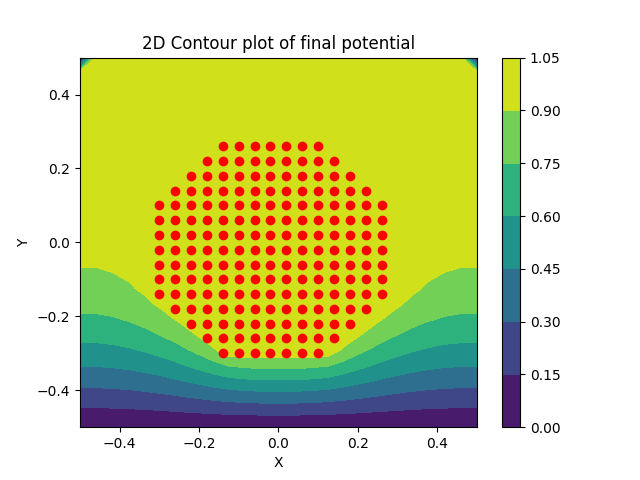
\includegraphics[scale=0.5]{Assgn5_plot5.png} 
\caption{Figure5}
\label{fig5}
\end{figure}

\begin{figure}[!tbh]
\centering
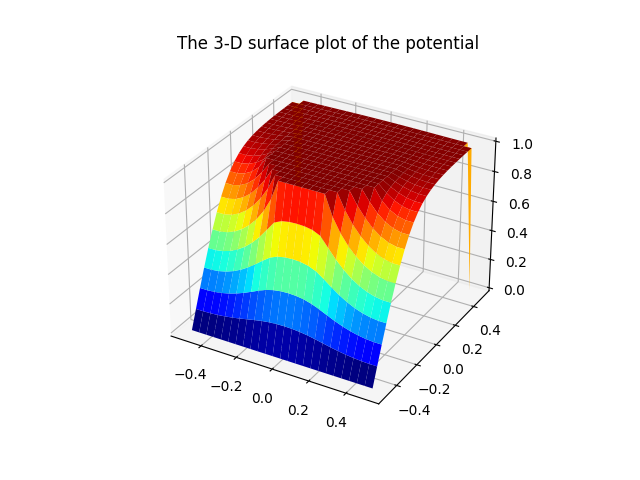
\includegraphics[scale=0.5]{Assgn5_plot6.png} 
\caption{Figure6}
\label{fig6}
\end{figure}


\subsection*{Finding current vectors}
The current vectors can be calculated as:
\begin{equation*}
 J(x,ij)=0.5*[\phi(i,j-1) - \phi(i,j+1)]
\end{equation*}
\begin{equation*} 
 J(y,ij)=0.5*[\phi(i-1,j) - \phi(i+1,j)]
\end{equation*}

We see that, the current fills the entire cross-section and then flows in the direction of the grounded electrode. Hardly any current flows out of the top part of the wire.
\begin{figure}[!tbh]
\centering
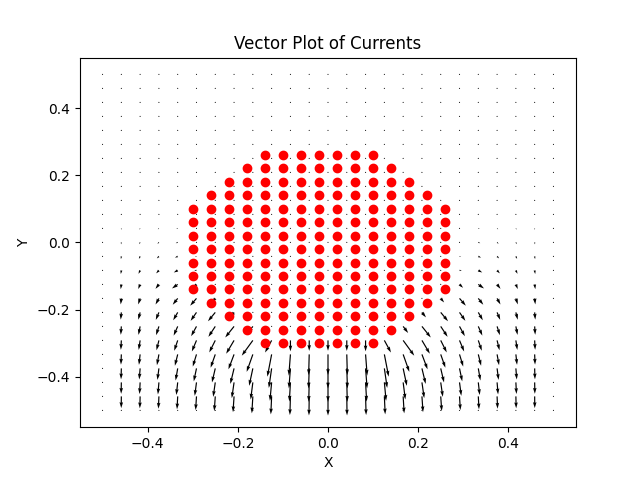
\includegraphics[scale=0.45]{Assgn5_plot7.png} 
\caption{Figure7}
\label{fig7}
\end{figure}

\section*{Conclusion}
We have used discrete differentiation to solve Laplace’s Equations.This method
of solving Laplace’s Equation is known to be one of the worst available. This is because of the very slow coefficient with which the error reduces.

\end{document}
